\documentclass{article}
\usepackage{amssymb}
\usepackage{graphicx}
\usepackage{amsmath}
\usepackage{url}
\usepackage{hyperref}
\usepackage{verbatim}
\usepackage{a4wide}
\usepackage[parfill]{parskip}

\begin{document}

\title{T-61.5060 Algorithmic Methods of Data Mining -- Programming Project}
\author{Rainer Kujala, rainer.kujala@aalto.fi \\ Olli-Pekka Koistinen, olli-pekka.koistinen@aalto.fi}

\maketitle

\section*{Introduction}

This programming project is a part of the Aalto University course T-61.5060 Algorithmic Methods of Data Mining.
The aim of the project is to study a large set of tweets collected from Twitter and develop algorithms that
are able to find exact or approximate nearest neighbors for separate query tweets.
A tweet is here defined as a set of terms that it includes, i.e., the order of the words and duplicate words are ignored.
The dataset contains about 15 million tweets, and 8.7 million unique terms.
The first 1000 tweets are considered as query tweets $q \in Q$, and the rest as database tweets $x \in D$.

To limit the amount of terms, three different dimension reduction strategies are considered:\\
$d$-frequent: Keep only the $d$ most frequent terms, and ignore the rest.\\
$d$-infrequent: Keep only the $d$ least frequent terms, and ignore the rest.\\
$d$-random: Keep $d$ random terms.

Let $t(x)$ denote the number of terms contained in tweet $x$. Given two tweets $x$ and $y$, the distance between
them is defined as the angle between the corresponding sets interpreted as vectors of $d$-dimensional binary space:

\begin{equation}
angle(x,y) = \arccos{{|x \cap y|}\over \sqrt{t(x)t(y)}}.
\label{eq:angle}
\end{equation}

Thus, the distance between similar tweets is equal 0, and the distance between tweets with no common terms equals $\pi \over 2$.

The first task is to examine the distribution of the number of term appearances in the dataset.
In the second task, a brute force algorithm is used to find an exact nearest neighbor for each query tweet $q \in Q$ from the database $D$.
The third task is to develop speedups for the exact nearest neighbor search,
and in the fourth task, approximate solutions are allowed to further speed up the algorithm.

The algorithms are implemented in Python programming language, and the programs are run in Triton cluster using \verb!pypy! interpreter
and a standardized Opteron processor.

\section*{Task 1 [preprocessing]}

In this task, we study the dataset by computing the number of tweets $n_t$ in which term $t$ appears.
In Fig.~\ref{fig:prepro-counts}, we show the distribution of $n_t$, i.e.,
the number of terms that appear in exactly $k$ tweets as a function of $k$.

\begin{figure}[h!]
\begin{center}
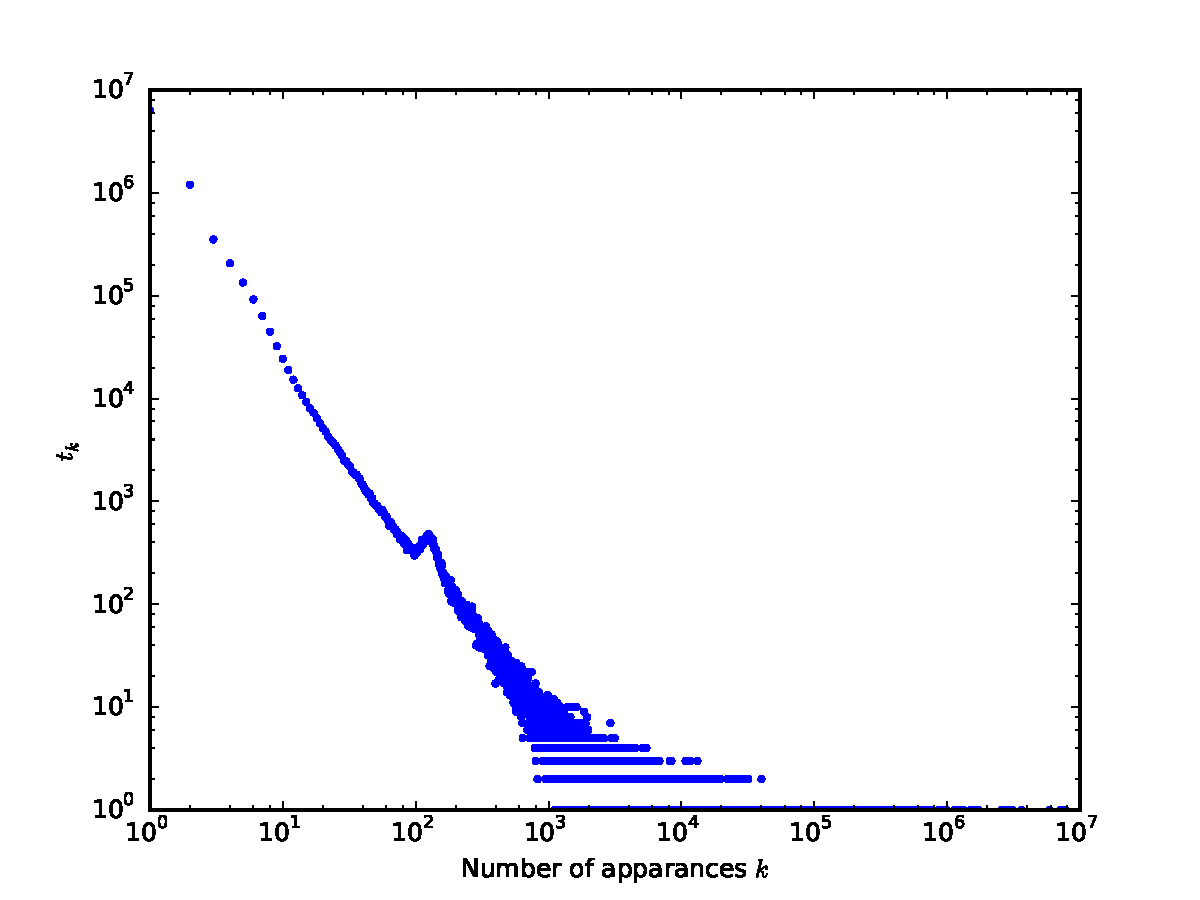
\includegraphics[width=0.7\linewidth]{{../figs/prepro_counts}.pdf}
\caption{Distribution of $n_t$.}
\label{fig:prepro-counts}
\end{center}
\end{figure}

Even though the underlying data is discrete, it is now convenient to plot the corresponding probability \emph{density}
function of the term counts in tweets. This is obtained by dividing the log-scale x-axis in 50 bins, counting the number of
tweets in each bin, and regarding the average probability density of the bin as the density of the bin center.
The plot of these densities is presented in Fig.~\ref{fig:prepro-pdf}, which shows also the power-law-like tail of the distribution.

\begin{figure}[h!]
\begin{center}
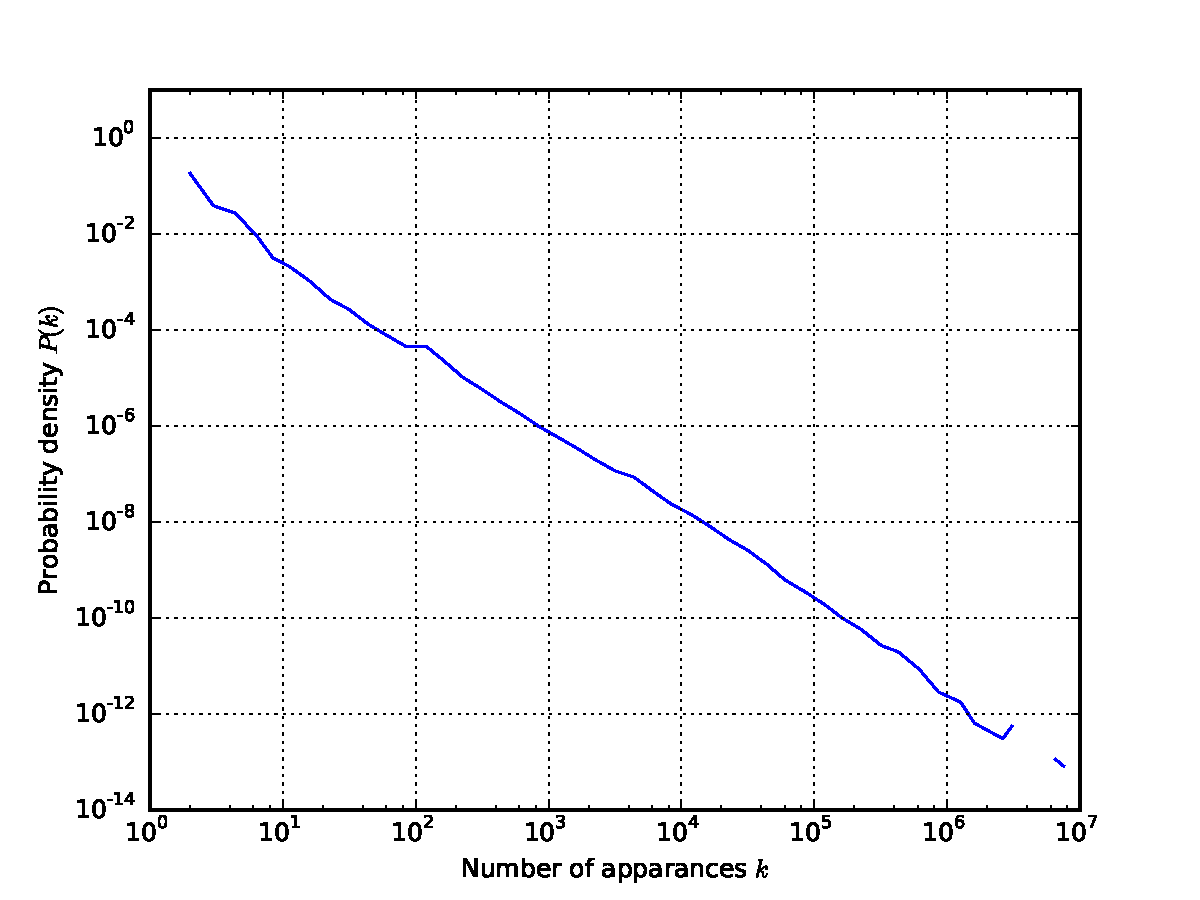
\includegraphics[width=0.7\linewidth]{{../figs/prepro_prob_density}.pdf}
\caption{Probability \emph{density} distribution of $n_t$.}
\label{fig:prepro-pdf}
\end{center}
\end{figure}

We define the cumulative $C(k)$ of a distribution to correspond to the \emph{complementary} cumulative distribution of a given probability distribution.
(The complementary cumulative distribution was used, as the standard CDF does not help out in understanding the data.)
Specifically, we defined the cumulative to correspond to $P(n_t\geq k)$, and it is presented in Fig.~\ref{fig:prepro-cumulative}.

\begin{figure}[h!]
\begin{center}
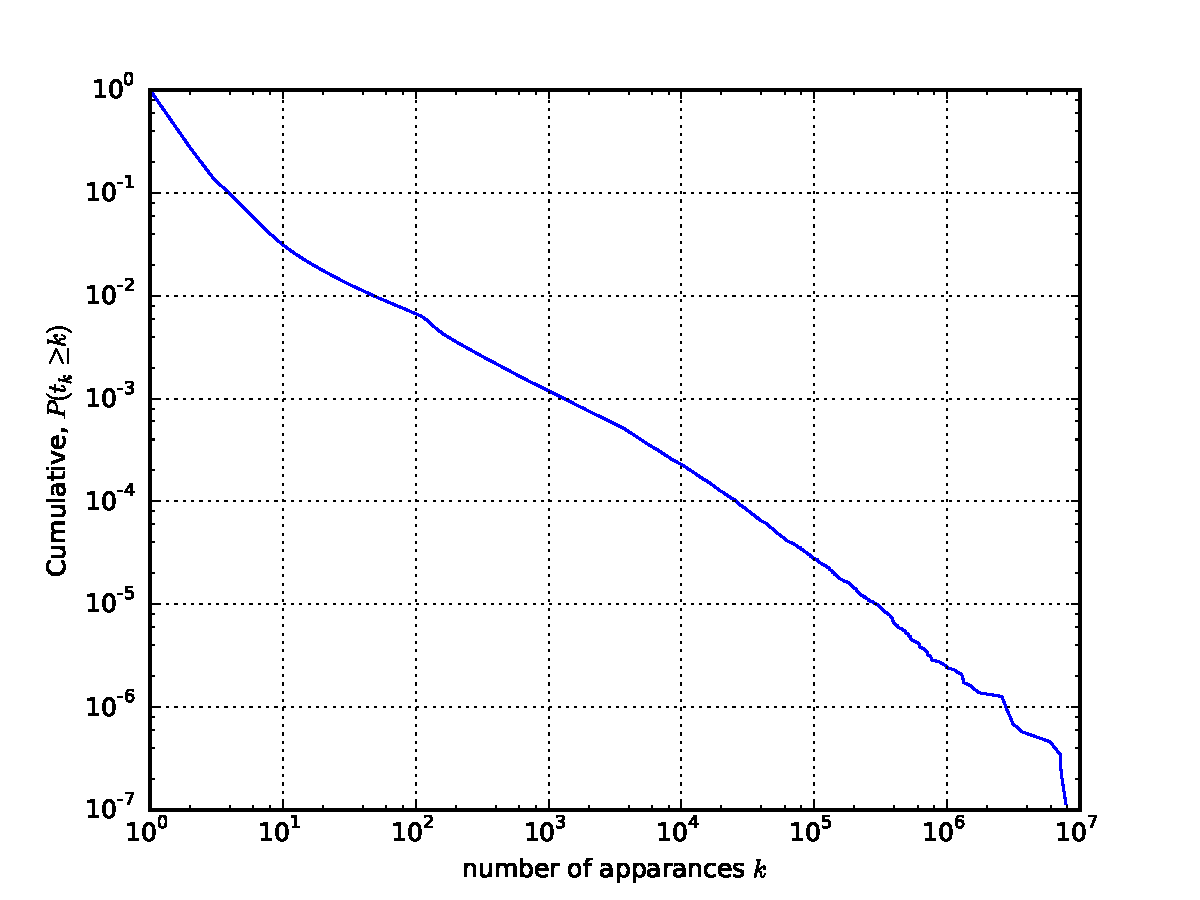
\includegraphics[width=0.7\linewidth]{{../figs/prepro_cumulative}.pdf}
\caption{Complementary cumulative distribution of $n_t$}
\label{fig:prepro-cumulative}
\end{center}
\end{figure}

Next we rename the terms as consecutive integers $1, 2, \dots, d$, so that $n_1 \geq n_2 \geq \dots \geq n_d$.
Fig.~\ref{fig:prepro-j-vs-nj} shows the number of tweets $n_j$ in which term $j$ appears as a function of $j$.
\begin{figure}[h!]
\begin{center}
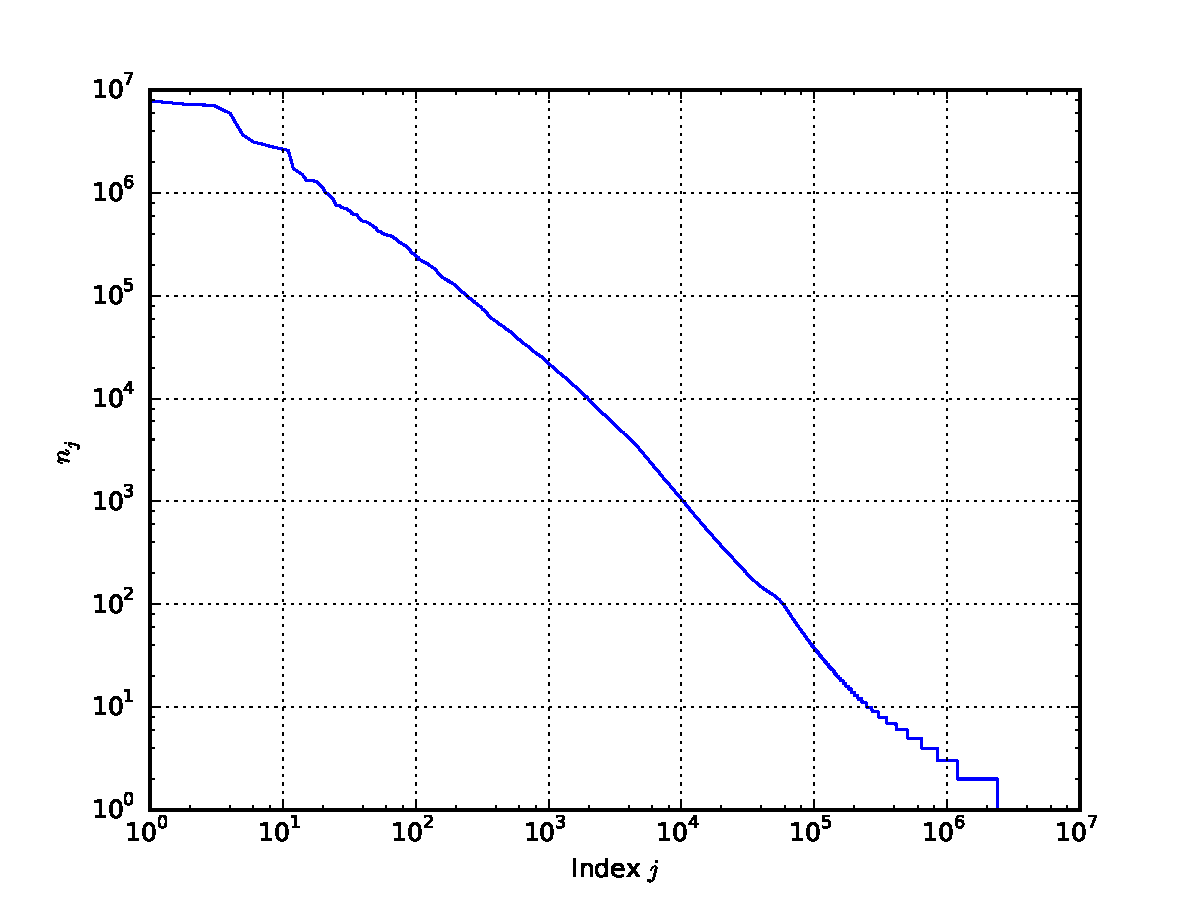
\includegraphics[width=0.7\linewidth]{{../figs/prepro_j_vs_nj}.pdf}
\caption{$n_j$ as a function of $j$}
\label{fig:prepro-j-vs-nj}
\end{center}
\end{figure}

All in all, the plots all tell the same story. The disribution of $n_t$ is broadly distributed (close to a power-law).
Most of the terms are extremely rare, whereas there also exist terms that appear in almost all tweets.




\section*{Task 2 [exact nearest neighbor --- brute force]}

In this task, we implement a brute force linear-search algorithm to find an exact nearest neighbor for a given query tweet $q$,
and perform full nearest-neighbor searches for $Q$, i.e., find a nearest neighbor for each query tweet $q \in Q$ from the database $D$,
using each three dimensionality-reduction strategies ($d$-frequent, $d$-infrequent, and $d$-random) with $d = 100 \cdot 2^j$, where $j = 0,2,4,...,14$.

The brute force algorithm simply goes through each database tweet $x \in D$, computes the distance between $q$ and $x$, and keeps a record for the
smallest distance so far. The distance is computed by returning $\pi \over 2$, if both the product of the lengths of $q$ and $x$ is equal to zero, and otherwise
by dividing the length of the intersection of $q$ and $x$ by the square root of product of the lengths of $q$ and $x$. Because the length of a tweet is
restricted, the time complexity of the distance computation is considered to be a constant. Thus, the time complexity of the brute force algorithm is
linear to the size of the database, $O(N)$.

The running times for the searches are presented in Fig.~\ref{fig:brute_force_runtimes_loglog}. From the figure, we can see that
the $d$-frequent dimensionality-reduction strategy does not reduce the running time as dramatically as the $d$-infrequent
and $d$-random strategies, when decreasing $d$. For the $d$-frequent strategy, there is no reduction in running time, when
$d > 10^4$, but with smaller $d$ the running time starts to decrease. Even if the running time reduces to about half with $d = 200$,
the reduction is not remarkable in log-log scale. For $d$-infrequent and $d$-random strategies, the scale of the running time reduces
clearly along with the scale of $d$, even though for the smallest dimensionality ($d = 200$) the running time is slightly longer than
for $d = 400$.

\begin{figure}[h!]
\begin{center}
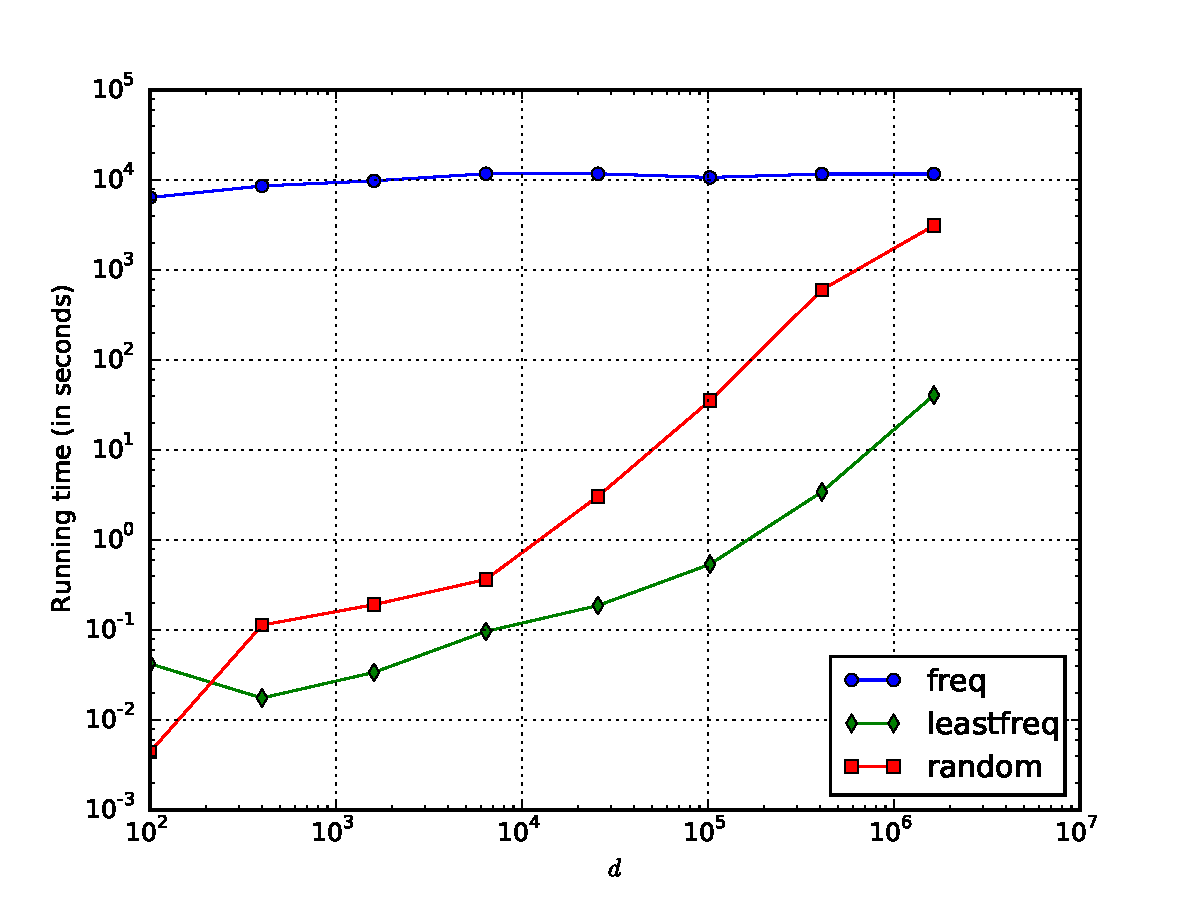
\includegraphics[width=0.7\linewidth]{{../figs/brute_force_runtimes_loglog}.pdf}
\caption{Running times for exact full nearest-beighbor searches obtained by a brute force algorithm.
The different colors represent the three dimensionality-reduction strategies: $d$-frequent (blue), $d$-infrequent (green), and $d$-random (red).
The running times are presented in log-log scale as a function of the dimensionality $d$.}
\label{fig:brute_force_runtimes_loglog}
\end{center}
\end{figure}

The behavior of the running times becomes quite intuitive, when taking into account that the dimensionality-reduction removes all terms of some tweets
and these empty tweets are removed from the database before running the nearest-neighbor search. Since the running time of the algorithm is linear to the size of
the database, the amount of empty tweets shows as a reduced running time. In case of the $d$-frequent strategy, the most frequent terms are reserved, which
is why there are not many empty tweets. In case of the $d$-random strategy, and especially $d$-infrequent strategy, where the most frequent terms are removed,
there are a lot of empty tweets, and the smaller is $d$, the more there are empty tweets and the more the running time is reduced.




\section*{Task 3 [exact nearest neighbor --- speedups]}

In this task, we develop speedups for the exact nearest-neighbor search algorithm, and compare the results with the brute force algorithm.
We implement two speedup tricks, which we explain next.

\subsection*{Trick 1: Immediate lookup table for identical tweets}

We noticed that in many cases (especially with low values of $d$), the database has multiple similar tweets.
Thus, it is also likely that the query tweets have exact matches with the database tweets.
To identify these exact matches, we preprocess the database by compiling first a hash table (i.e., a Python dictionary object), whose keys are the tweets (hashed as a sorted tuple) and values are the indices of those tweets.
\footnote{Note that by using this kind of hash table, we could have also removed all the duplicates from the initial data sets. However, this was not implemented due to time constraints.}

Having this hash table at our disposal, we can immediately find the nearest neighbors for some of the tweets, but not for all.
For the rest of the query tweets, we have to search the exact nearest neighbors in another way, which corresponds to the trick 2.

\subsection*{Trick 2: Looping only through tweets that have at least one common term as the query tweet}

As was pointed out also in the project description, any two tweets with an angle smaller than $\pi \over 2$ must share at least one common term.
Given a query tweet for which no exact match could be found, we thus want to loop only over those tweets that have one or more common terms with the query tweet.
To achieve this goal, we build a hash table which maps each term to a list of database tweets that contain that term.
These hash tables are created separately for each of the $3 \dot 7 = 24$ data dimensionality reduction strategies.

Then, given a query tweet, we first obtain all database tweets that contain any of the terms of the query tweet.
When obtaining the candidate database tweets, we also compute how many common terms each of the database tweets have in common with the query tweet.
This enables us then to loop over the candidate tweets in a prioritized order, so that we first go through tweets that have the largest number of common terms with the query tweet.
This sorting of the candidate tweets is implemented only partially by grouping the tweets based on the number of common terms with the query tweet,
and thus its time complexity is linear with respect to the number of candidate tweets.

The actual reason to loop over the query tweets in a prioritized manner is that we could apply an early stopping criterion for the nearest-neighbor search.
This early stopping criterion is based on the following notion: Given a query tweet $q$ of length $t(q)$ and knowing that all of the remaining candidate tweets can have at most $c$ common terms with $q$,
the minimum distance between $q$ and any other query tweet is achieved when a database tweet contains only those $c$ common terms.
Given $c$ and $t(x)$, the lower bound $l$ for the minimum distance between the query tweet and a remaining database tweet can be obtained directly from Eq.~\ref{eq:angle} and equals

\begin{equation}
l(t(x), c) = \arccos{{c}\over \sqrt{c t(x)}}.
\label{eq:ubound}
\end{equation}

This lower bound can then be utilized in two ways:
\begin{enumerate}
\item If we find a tweet whose distance to the query tweet equals to the current lower bound, we have found an exact nearest neighbor.
\item Consider the case where we start going through a new group of candidates all having $c'$ common terms with the query tweet.
If the distance between the query tweet and its nearest neighbor so far is smaller than or equal to the new lower bound $l(t(x), c')$,
we have already found an exact nearest neighbor for the query tweet $x$.
\end{enumerate}

\subsection*{Results}

The speedups obtained are presented in Fig.~\ref{fig:speedups_loglog}. Let us go through the speedup curves separately for each of the dimensionality-reduction strategies:
\begin{itemize}
\item \verb!freq!: In the case, where we use the most frequent terms in the database, we have speedups $> 1$ only when $d < 10^4$.
After this limit, the overhead caused by our algorithm takes over and the running times are even slower than with the brute force algorithm.
\item \verb!leastfreq!: With the least frequent terms, we obtain significant speedup when the number of the terms considered is larger than $\approx 10^4$.
With small values of $d$, the additional overhead from our improved algorithm (compared to the brute force algorithm) seems to just slow down the computations.
This is understandable, as with low values of $d$ the size of the data set is very small.
\item \verb!random!: When using the random terms, we obtain significant speedups with all possible values of $d$.
Note that with small values of $d$, the speedup fluctuates heavily due to the relatively small number of terms used.
With the largest value of $d$, we can also notice a drop in the speedups with respect to the increasing trend of speedups.
\end{itemize}

\begin{figure}[h!]
\begin{center}
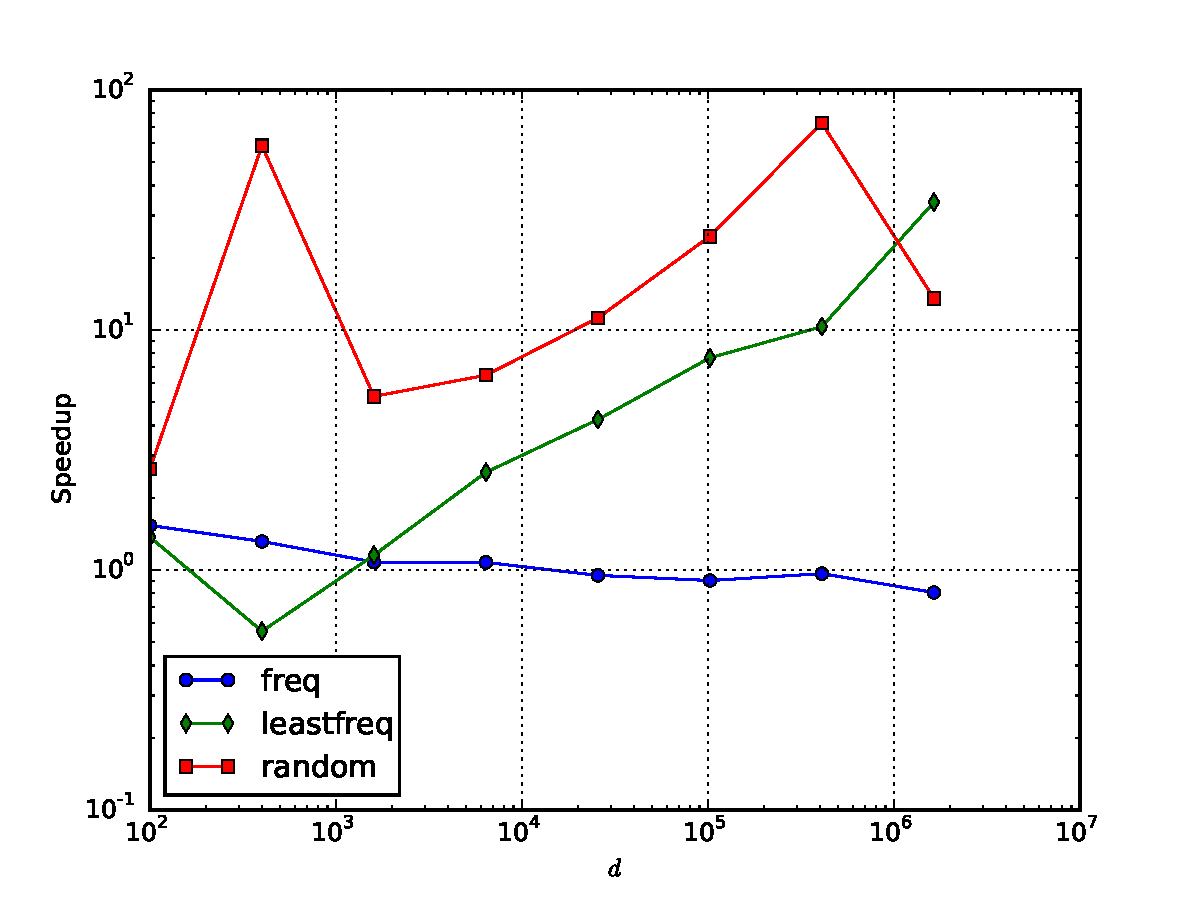
\includegraphics[width=0.7\linewidth]{{../figs/speedups_loglog}.pdf}
\caption{The obtained speedups of the improved nearest-neighbor search algorithm with respect to the brute force nearest-neighbor search.
The different colors represent the three dimensionality-reduction strategies: $d$-frequent (blue), $d$-infrequent (green), and $d$-random (red).
The speedups are presented in log-log scale as a function of the dimensionality $d$.}
\label{fig:speedups_loglog}
\end{center}
\end{figure}


\subsection*{Discussion of the results}

For the datasets created using the least frequent and random terms, our improved algorithm mostly performed better than the brute force algorithm.
However, when using the most frequent terms, we only obtained speedups when $d$ was kept small.
We speculate that the reasons, why we could not obtain any speedup with larger values of $d$, may be due to the following reasons:

\begin{enumerate}
\item The algorithmic overhead (i.e., obtaining candidates and sorting the data) becomes significant, when the size of the database is increased.
We have not performed thorough theoretical investigations, but for example the time required for obtaining all possible candidates and sorting them (approximately in linear time) does take a considerable amount of time.
\item When looping over the candidates, we need to access the memory in a random fashion, which can make a significant difference, when compared for example to the brute force algorithm, where all data is treated sequentially.
\item For running our codes, we used \verb!pypy!. In our code, we utilized large python dictionaries with which \verb!pypy!, however, has had some performance issues (see, e.g., ~\url{http://pypy.org/performance.html}).
In our runs, we experienced also huge memory requirements by our code, even though the datasets and the indices themselves were not that large when stored on disk.
\item Details of the implementation: Our speedup algorithm reduces heavily the number of calls to the function computing the distance between two tweets in all the cases above.
If the computation of the distance function was more time consuming (with respect to the other parts of our algorithm), we would have naturally obtained larger speedups in each of the previous cases.
\end{enumerate}




\section*{Task 4 [approximate nearest neighbor]}

In this task, we aim for further speedups by developing an approximate nearest-neighbor search algorithm.
This requires only a tiny change to our exact search algorithm.
Instead of using the lower bound $l$ (for the distance to a remaining database tweet candidate) in the two stopping criteria,
we now use $(1 + \epsilon) l$ instead (where $\epsilon \in \{0.5, 0.2\}$ is the allowed relative error as provided in the project description).
This enables us then to stop the iteration over candidates sooner, which thus necessarily yields larger speedups.

The obtained speedups are presented in Figs.~\ref{fig:approx_speedups_loglog_1.5} and ~\ref{fig:approx_speedups_loglog_1.2} for $\epsilon = 0.5$ and $\epsilon = 0.2$, respectively.
In general, the speedups are slightly higher than with the exact search algorithm.
With large databases (using $d$-frequent dimensionality reduction with large $d$), the same problems persist as with the exact search algorithm:
most of the running time goes into the sorting and collecting of the candidates, and thus we do not obtain almost any speedup compared to the exact search algorithm.

\begin{figure}[h!]
\begin{center}
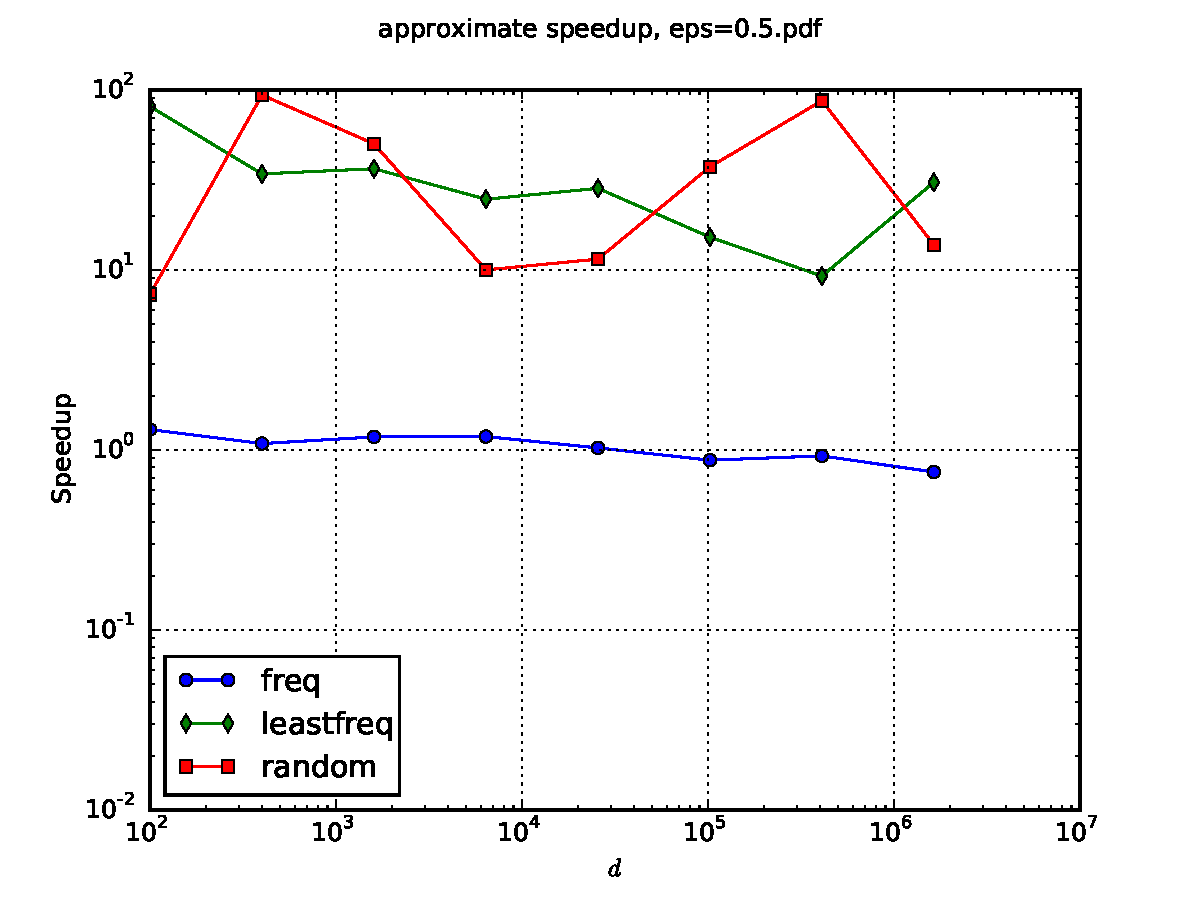
\includegraphics[width=0.7\linewidth]{{../figs/speedups_approx_1.5_loglog}.pdf}
\caption{The obtained speedups of the approximate nearest-neighbor search algorithm ($\epsilon = 0.5$) with respect to the brute force nearest-neighbor search.
The different colors represent the three dimensionality-reduction strategies: $d$-frequent (blue), $d$-infrequent (green), and $d$-random (red).
The speedups are presented in log-log scale as a function of the dimensionality $d$.}
\label{fig:approx_speedups_loglog_1.5}
\end{center}
\end{figure}

\begin{figure}[h!]
\begin{center}
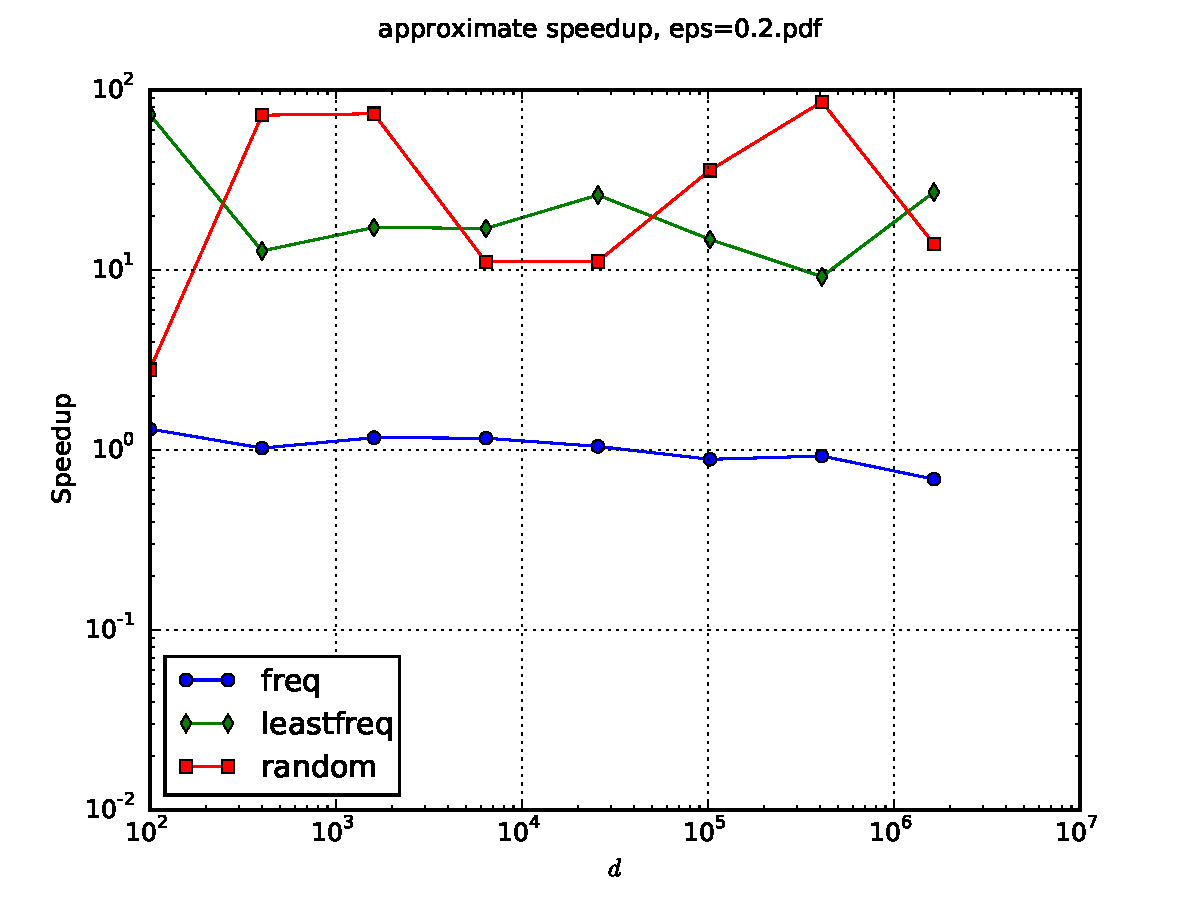
\includegraphics[width=0.7\linewidth]{{../figs/speedups_approx_1.2_loglog}.pdf}
\caption{The obtained speedups of the approximate nearest-neighbor search algorithm ($\epsilon = 0.2$) with respect to the brute force nearest-neighbor search.
The different colors represent the three dimensionality-reduction strategies: $d$-frequent (blue), $d$-infrequent (green), and $d$-random (red).
The speedups are presented in log-log scale as a function of the dimensionality $d$.}
\label{fig:approx_speedups_loglog_1.2}
\end{center}
\end{figure}

We also compute the mean approximation error $\langle e \rangle$ averaged over all query tweets.
As a measure of the approximation error $e$, we use
\begin{equation}
e = \frac{\alpha^* - \alpha}{\alpha},
\end{equation}where $\alpha$ is the distance between the query tweet and its exact nearest neighbor, and $\alpha^*$ is the distance between the query tweet and the approximate nearest neighbor returned by our algorithm.
If $\alpha = 0$ (and in our algorithm then also $\alpha^* = 0$ due to the immediate lookup of identical tweets), we define $e$ to be zero.

The mean approximation errors for each dimensionality-reduction strategy are shown in Figs.~\ref{fig:approx_error_1.5} and \ref{fig:approx_error_1.2} for $\epsilon = 0.5$ and $\epsilon = 0.2$, respectively.
As our algorithm is now rather strict (i.e., it does not allow the approximation error of \emph{any} tweet to be above $\epsilon$), our mean approximation errors remain low for each of the cases.

\begin{figure}[h!]
\begin{center}
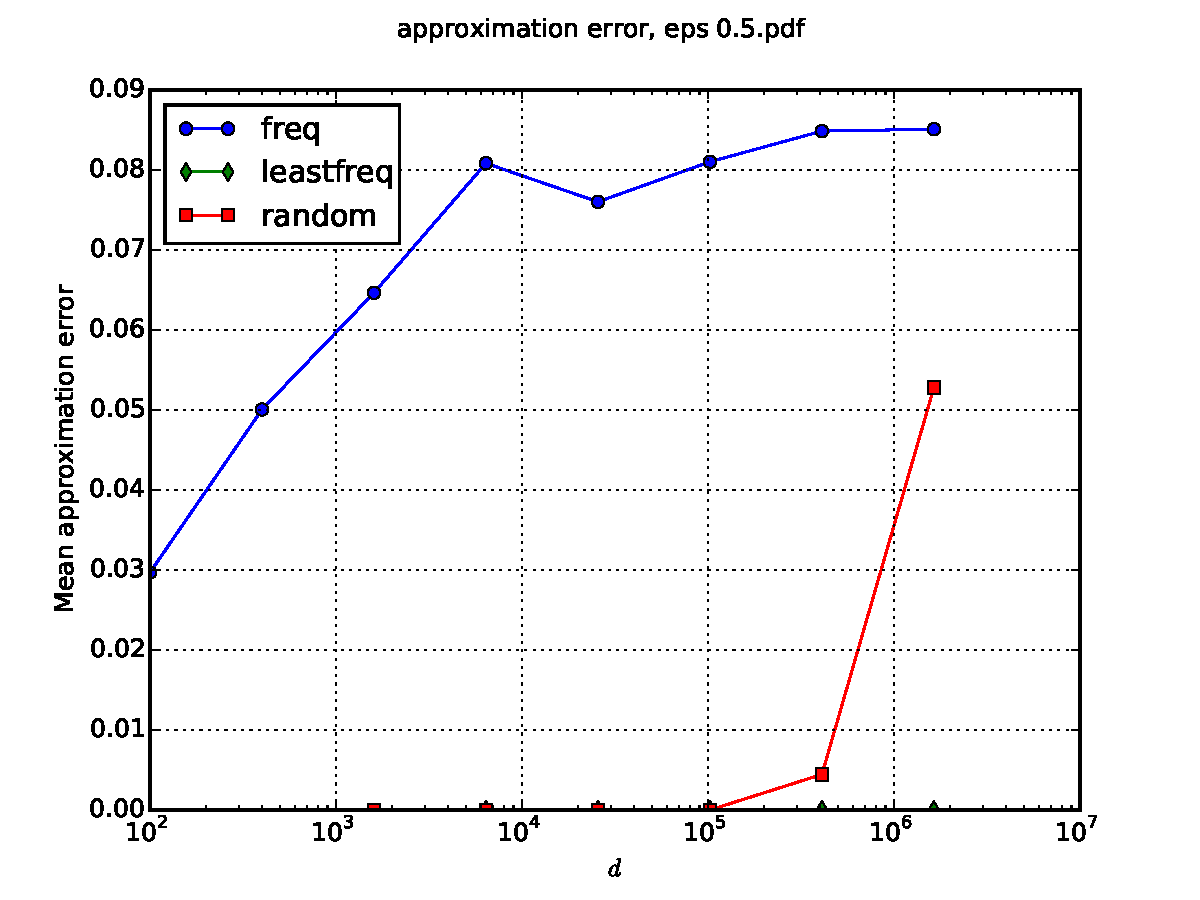
\includegraphics[width=0.7\linewidth]{{../figs/approximation_error_eps_1.5_loglog}.pdf}
\caption{The mean approximation errors with $\epsilon = 0.5$.
The different colors represent the three dimensionality-reduction strategies: $d$-frequent (blue), $d$-infrequent (green), and $d$-random (red).
The errors are presented as a function of the dimensionality $d$.}
\label{fig:approx_error_1.5}
\end{center}
\end{figure}

\begin{figure}[h!]
\begin{center}
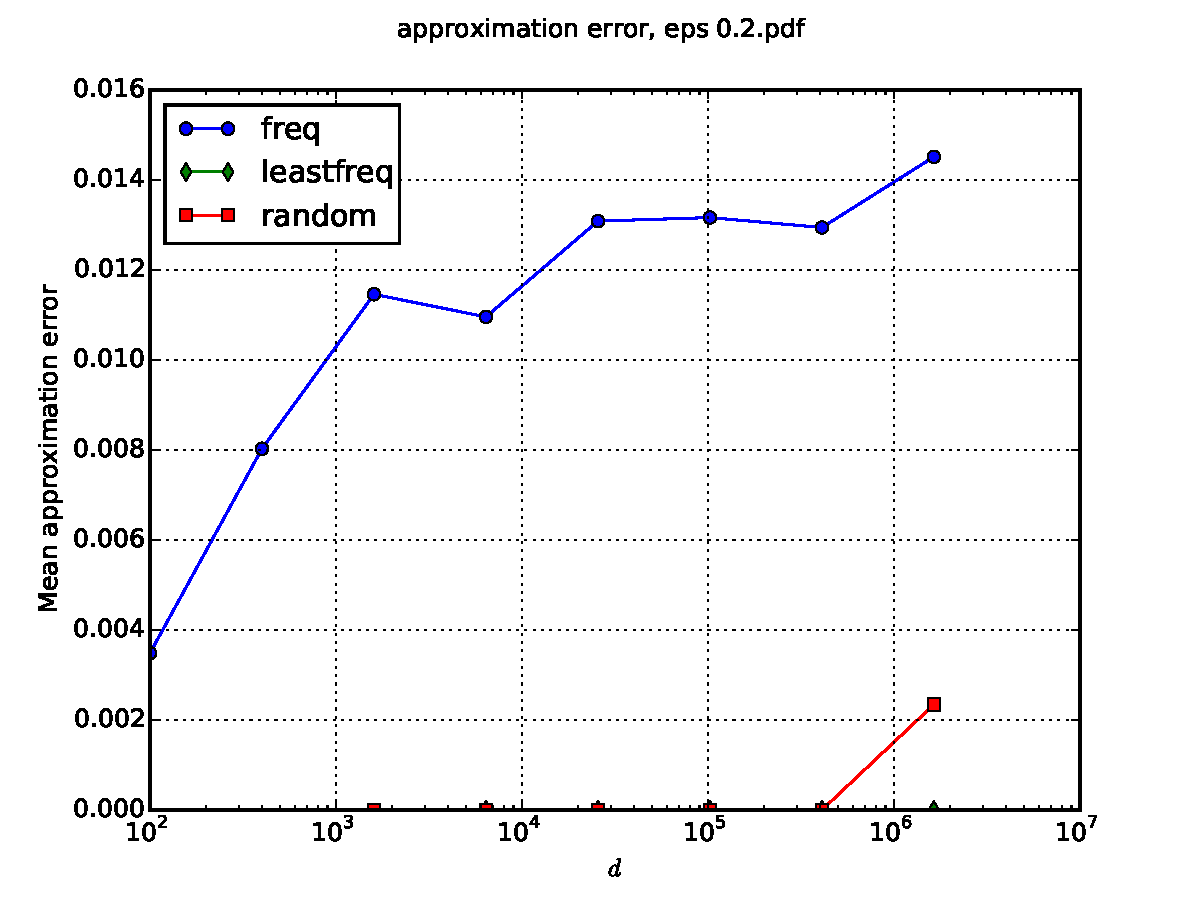
\includegraphics[width=0.7\linewidth]{{../figs/approximation_error_eps_1.2_loglog}.pdf}
\caption{The mean approximation errors with $\epsilon = 0.2$.
The different colors represent the three dimensionality-reduction strategies: $d$-frequent (blue), $d$-infrequent (green), and $d$-random (red).
The errors are presented as a function of the dimensionality $d$.}
\label{fig:approx_error_1.2}
\end{center}
\end{figure}

\subsection*{Discussion}

When comparing the speedups of our approximate algorithm to the speedups obtained with the exact search algorithm, we did not reach remarkable advantage.
This result highlights a need for a yet faster algorithm.
One such candidate method would be, e.g., the locality sensitive hashing (LSH),
which in this case could have been implemented by hashing the tweets based on which side of random planes they reside~\footnote{See, e.g., \url{http://en.wikipedia.org/wiki/Locality-sensitive_hashing\#Random_projection}.}
We speculate, that with appropriate tuning, the LSH-approach could have outperformed our algorithm.
However, having had problems with working even a small number of hash tables, we refrained from implementing a working LSH algorithm in this project.

\end{document}
